\textbf{Pour cette première partie, aucune justification n'est demandée et une seule réponse est possible par question. Pour chaque question, reportez son numéro sur votre copie et indiquez votre réponse.}\par
Une réponse fausse ou l'absence de réponse n'enlève aucun point.

\vspace{.8em}

\subsection*{Question 1}

Un lycée compte 500 élèves. 20\% des élèves sont externes. Le nombre d'externes est :
\begin{center}
\begin{tabularx}{.92\linewidth}{XXXX} A. 10 & B. 20 & C. 100 & D. 520\end{tabularx}\end{center}

\begin{color}{blue}Solution :\par
$20~\%\times 500 = \dfrac{20}{100}\times 500 = \dfrac{20}{100}\times 100 \times 5 = 20 \times 5 = 100$

\textbf{C. 100}
\end{color}

\subsection*{Question 2}

Un lycée compte 500 élèves. L'effectif augmente de 5\% l'année suivante. Le nombre d'élèves est donc multiplié par :
\begin{center}
\begin{tabularx}{.92\linewidth}{XXXX} A. 5 & B. 1,05 & C. 0,05 & D. 25\end{tabularx}
\end{center}

\begin{color}{blue}Solution :\par

Le coefficient multiplicateur s'obtient avec le calcul : $1+5~\% = 1 + \dfrac{5}{100} = 1,05$

\textbf{B. 1,05}
\end{color}

\subsection*{Question 3}

$4\times\dfrac{2}{3}=$
\begin{center}
\begin{tabularx}{.92\linewidth}{XXXX} A. $\dfrac{8}{3}$ & B. $\dfrac{8}{12}$ & C. $\dfrac{24}{3}$ & D. $\dfrac{24}{9}$\end{tabularx}
\end{center}

\begin{color}{blue}Solution :\par
$4\times\dfrac{2}{3} = \dfrac{4\times 2}{3} = \dfrac{8}{3}$

\textbf{A. $\dfrac{8}{3}$} ou \textbf{D. car $\dfrac{8}{3} = \dfrac{8\times 3}{3\times 3} = \dfrac{24}{9}$}
\end{color}

\subsection*{Question 4}

Quelle équation admet deux solutions réelles ?
\begin{center}
\begin{tabularx}{.92\linewidth}{XXXX} A. $2x=-1$ & B. $x^2=-1$ & C. $x^2=4$ & D. $\dfrac{x}{2}=4$\end{tabularx}
\end{center}

\begin{color}{blue}Solution :\par
$2x=-1 \iff x=-\dfrac{1}{2}$

$x^2>0$ pour tout réel $x$ donc $x^2=-1$ n'a pas de solution réelle

$\dfrac{x}{2}=4\iff x=8$

$x^2=4$ a deux solutions $-2$ et $2$ ($(-2)^2 = 4$ et $2^2 = 4$)

\textbf{C. $x^2=4$}
\end{color}


\subsection*{Question 5}

\begin{center}
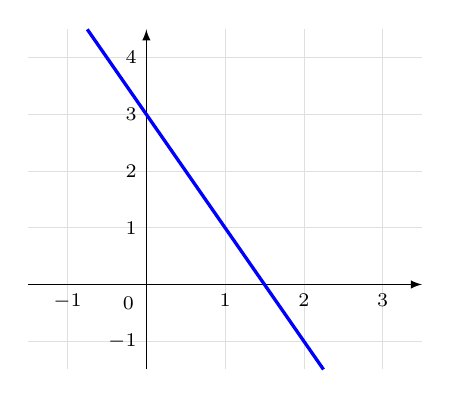
\begin{tikzpicture}[xscale=1,yscale=.72]
\draw[step=1cm,gray!25,very thin] (-1.5,-1.5) grid (3.5,4.5);
\draw[-latex] (-1.5,0)--(3.5,0);
\draw[-latex] (0,-1.5)--(0,4.5);
\foreach \x in {-1,1,2,3}
  \node[below] at (\x,0) {\scriptsize $\x$};
\foreach \y in {-1,1,2,3,4}
  \node[left] at (0,\y) {\scriptsize $\y$};
\node[below left=1pt] at (0,0) {\scriptsize 0};
\draw[very thick,blue] (-0.75,4.5)--(2.25,-1.5);
\end{tikzpicture}
\end{center}

L'équation de la droite représentée ci-dessus est :
\begin{center}
\begin{tabularx}{.92\linewidth}{XXXX} A. $y=-0,5x+1,5$ & B. $y=-2x+1,5$ & C. $y=2x+3$ & D. $y=-2x+3$\end{tabularx}
\end{center}

\begin{color}{blue}Solution :\par
L'équation réduite d'une droite non parallèle à l'axe des ordonnées est de la forme $y=mx+p$

Le point de coordonnées $(0;3)$ appartient à la droite. Ainsi $p=3$.

Le point de coordonnées $(1;1)$ appartient à la droite. $1 = m\times 1 + 3$ et donc $m=\dfrac{1-3}{1} = -2$.

\textbf{D. $y=-2x+3$}
\end{color}

\subsection*{Question 6}

On considère la fonction $f$ définie sur $\mathbb{R}$ par $f(x)=x(3x-6)$.\par
L'image de $-2$ par cette fonction est :
\begin{center}
\begin{tabularx}{.92\linewidth}{XXXX} A. $-14$ & B. $-24$ & C. $24$ & D. $-48$\end{tabularx}
\end{center}

\begin{color}{blue}Solution :\par
$f(-2)=(-2)\times(3\times(-2)-6) = (-2)\times(-6-6) =(-2)\times(-12) = 24 $

\textbf{C. $24$}
\end{color}

\subsection*{Question 7}

On considère la fonction $f$ définie sur $\mathbb{R}$ par $f(x)=x(3x-6)$.\par
Le nombre 0 admet :
\begin{center}
\begin{tabularx}{.92\linewidth}{XXXX} A. Deux antécédents : 0 et 2 & B. Un seul antécédent : 0 \\ C. Un seul antécédent : $-18$ & D. Deux antécédents : 0 et $-2$\end{tabularx}
\end{center}

\begin{color}{blue}Solution :\par
$f(2)=2\times(3\times 2-6) = 2\times(6-6) =2\times 0 = 0 $

$f(0)=0\times(3\times 0 -6) = 0 $

\textbf{A. Deux antécédents : 0 et 2}
\end{color}


\subsection*{Question 8}

On considère la représentation graphique d'une fonction $f$ polynôme du second degré, définie sur $\mathbb{R}$.
\begin{center}
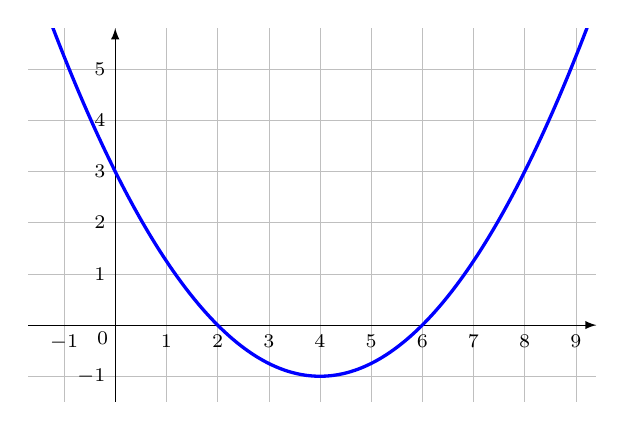
\begin{tikzpicture}[scale=.65]
\draw[step=1cm,gray!50,very thin] (-1.7,-1.5) grid (9.4,5.8);
\draw[-latex] (-1.7,0)--(9.4,0);
\draw[-latex] (0,-1.5)--(0,5.8);
\foreach \x in {-1,1,2,3,4,5,6,7,8,9}
  \node[below] at (\x,0) {\scriptsize $\x$};
\foreach \y in {-1,1,2,3,4,5}
  \node[left] at (0,\y) {\scriptsize $\y$};
\node[below left=-1pt] at (0,0) {\scriptsize 0};
\begin{scope}
\clip (-1.7,-1.5) rectangle (9.4,5.8);
\draw[very thick,blue,domain=-2:10,samples=200]
  plot (\x,{0.25*(\x-2)*(\x-6)});
\end{scope}
\end{tikzpicture}
\end{center}
Le tableau de signes de cette fonction $f$ est :

A

\begin{tikzpicture}
\tkzTabInit[lgt=2.5, espcl=2]{$x$ / 1, {Signe de $f(x)$} / 1}{${-\infty}$, ${3}$, ${2}$, ${6}$, ${+\infty}$}
\tkzTabLine{,-,z,+,z,-,z,+,}
\end{tikzpicture}

B

\begin{tikzpicture}
\tkzTabInit[lgt=2.5, espcl=2]{$x$ / 1, {Signe de $f(x)$} / 1}{${-\infty}$, ${}$, ${4}$, ${}$, ${+\infty}$}
\tkzTabLine{,-,,,z,,,+,}
\end{tikzpicture}

C

\begin{tikzpicture}
\tkzTabInit[lgt=2.5, espcl=2]{$x$ / 1, {Signe de $f(x)$} / 1}{${-\infty}$, ${2}$, ${}$, ${6}$, ${+\infty}$}
\tkzTabLine{,-,z,,+,,z,-,}
\end{tikzpicture}

D

\begin{tikzpicture}
\tkzTabInit[lgt=2.5, espcl=2]{$x$ / 1, {Signe de $f(x)$} / 1}{${-\infty}$, ${2}$, ${}$, ${6}$, ${+\infty}$}
\tkzTabLine{,+,z,,-,,z,+,}
\end{tikzpicture}

\begin{color}{blue}Solution :\par
\begin{tikzpicture}
\tkzTabInit[lgt=2.5, espcl=2]{$x$ / 1, {Signe de $f(x)$} / 1}{${-\infty}$, ${2}$, ${}$, ${6}$, ${+\infty}$}
\tkzTabLine{,+,z,,-,,z,+,}
\end{tikzpicture}

\textbf{D}
\end{color}


\subsection*{Question 9}

Une course automobile consiste à parcourir 20 tours d'une piste de \np{4500}~mètres. La distance totale de la course est :
\begin{center}
\begin{tabularx}{.92\linewidth}{XXXX} A. \np[m]{9000} & B. \np[km]{9} & C. \np[km]{90} & D. \np[km]{45}
\end{tabularx}
\end{center}

\begin{color}{blue}Solution :\par
$\np[m]{4500} = \np[km]{4.5}$ et $20\times \np{4.5}=90$

\textbf{C. \np[km]{90}}
\end{color}


\subsection*{Question 10}

Un élève a obtenu la note de 10/20 à un devoir coefficienté 2 et la note de 16/20 à un devoir coefficienté 1. La moyenne de l'élève est :
\begin{center}
\begin{tabularx}{.92\linewidth}{XXXX} A. 11 & B. 12 & C. 13 & D. 14\end{tabularx}
\end{center}

\begin{color}{blue}Solution :\par
Calcul de la moyenne pondérée par les coefficients : $\dfrac{2\times 10 +  1\times 16}{2+1} = \dfrac{36}{3} = 12$

\textbf{B. 12}
\end{color}

\subsection*{Question 11}

Le tableau ci-dessous donne la répartition des achats d'aspirateurs d'un magasin d'électroménager.
\begin{center}
\renewcommand{\arraystretch}{1.25}
\begin{tabular}{|c|c|c|c|}\hline
& Avec sac & Sans sac & Total\\\hline
Avec fil & 102 & 58 & 160\\\hline
Sans fil & 20 & 70 & 90\\\hline
Total & 122 & 128 & 250\\\hline
\end{tabular}
\end{center}

On interroge au hasard un client parmi ceux qui ont acheté un aspirateur sans fil.\par
La probabilité que ce client ait acheté un aspirateur avec sac est :
\begin{center}
\begin{tabularx}{.92\linewidth}{XXXX} A. $\dfrac{20}{70}$ & B. $\dfrac{20}{90}$ & C. $\dfrac{20}{250}$ & D. $\dfrac{20}{122}$\end{tabularx}
\end{center}

\begin{color}{blue}Solution :\par
La population de référence est l'ensemble des clients qui ont acheté un aspirateur sans fil. On considère donc l'effectif de 90. Parmi ceux-ci 70 ont acheté un aspirateur sans sac. Donc 20 ($90-70$) en ont acheté un avec sac.

La probabilité cherchée est : $\dfrac{20}{90}$

\textbf{B. $\dfrac{20}{90}$}
\end{color}


\subsection*{Question 12}

Le diagramme ci-dessous donne la répartition des ventes d'un concessionnaire automobile.
\begin{center}
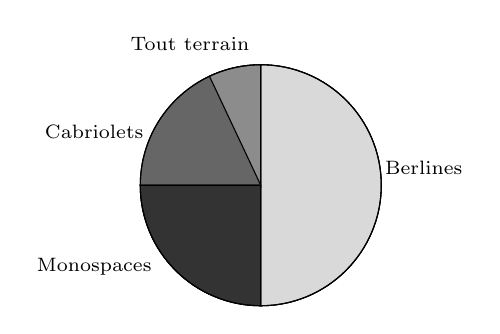
\begin{tikzpicture}[scale=.9]
\draw[fill=black!60] (0,0) -- (-180:1.7) arc(-180:270:1.7) -- cycle;
\draw[fill=black!15] (0,0) -- (90:1.7) arc(90:-90:1.7) -- cycle;
\draw[fill=black!80] (0,0) -- (-90:1.7) arc(-90:-180:1.7) -- cycle;
\draw[fill=black!45] (0,0) -- (115.2:1.7) arc(115.2:90:1.7) -- cycle;
\draw (0,0) circle(1.7);
\node at (2.3,.25) {\scriptsize Berlines};
\node at (-2.35,-1.15) {\scriptsize Monospaces};
\node at (-2.35,.75) {\scriptsize Cabriolets};
\node at (-1,2.0) {\scriptsize Tout terrain};
\end{tikzpicture}
\end{center}

Quel pourcentage des ventes représentent les véhicules cabriolets ?
\begin{center}
\begin{tabularx}{.92\linewidth}{XXXX} A. 52\% & B. 12\% & C. 18\% & D. 30\%\end{tabularx}
\end{center}

\begin{color}{blue}Solution :\par
Pour les berlines : la moitié soit 50~\%.

Pour les monospaces : le quart soit 25~\%.

Pour le reste, les cabriolets et les tout terrain, cela représente donc 25~\%. Il y a plus de cabriolets vendus que de tout terrain. Donc on choisit 18~\%.

\textbf{C. 18\%}
\end{color}
